\documentclass[UTF8]{ctexart}
\usepackage{datetime}
\usepackage{geometry}
\usepackage{array}
\usepackage{graphicx}
% 封面
\geometry{a4paper,left=1cm,right=2cm,top=1cm,bottom=1cm}
\title{\Huge 电工电子实验中心}
\author{\Large 实验报告}
\begin{document}
\maketitle
\vspace{6\baselineskip}
\renewcommand\arraystretch{1.5}
\begin{table}[h]
    \centering
    \Large
    \setlength{\tabcolsep}{5mm}{
        \begin{tabular}{rcrc}
            课程名称: & 数字电子技术 & 实验项目: & 数据选择器与译码器的应用 \\

            姓名:     & xxx       & 学号:     & xxxxxxxxx    \\

            班级:     & xxxxxxx      & 日期:     & \today       \\

            地点:     & 3313         & 成绩:     &              \\
        \end{tabular}}
\end{table}

\vspace{10\baselineskip}

\centering
南京航空航天大学 \\
\newpage


% 内容页
\begin{enumerate}
    \large
    \vspace{1\baselineskip}
    \item  预习:
          \begin{itemize}
              \item 设计任务:
                    \begin{itemize}
                        \item [1.]  芯片的测试。
                              要求:
                              \begin{itemize}
                                  \item [1)] 接电源。 
                                  \item [2)] 接使能端。
                                  \item [3)] 输入管脚选1组数据。
                                  \item [4)] 测量输出端,看是否正确。
                                  \item 对于74LS138,输出   应该为低电平,其余输出引脚为高电平。对于74LS153,输出Y=D3,D3悬空,为高电平。
                              \end{itemize}
                        \item [2.]  用74LS138和74LS20实现一位全加器

                        \begin{center}
                            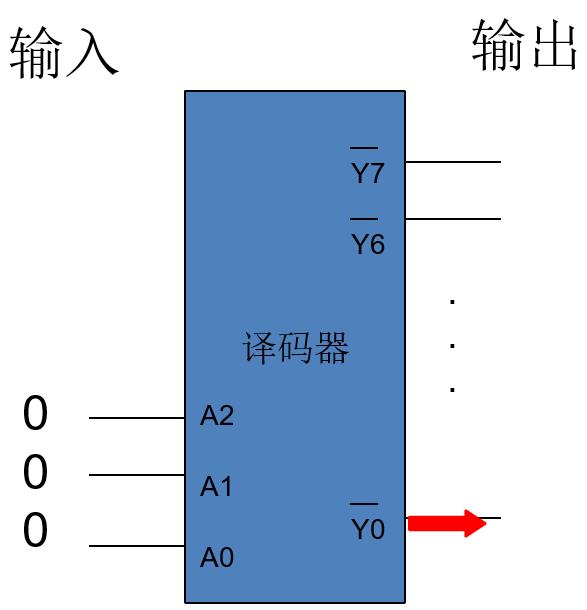
\includegraphics[scale=0.4]{7.png}
                            \label{fig:label}
                            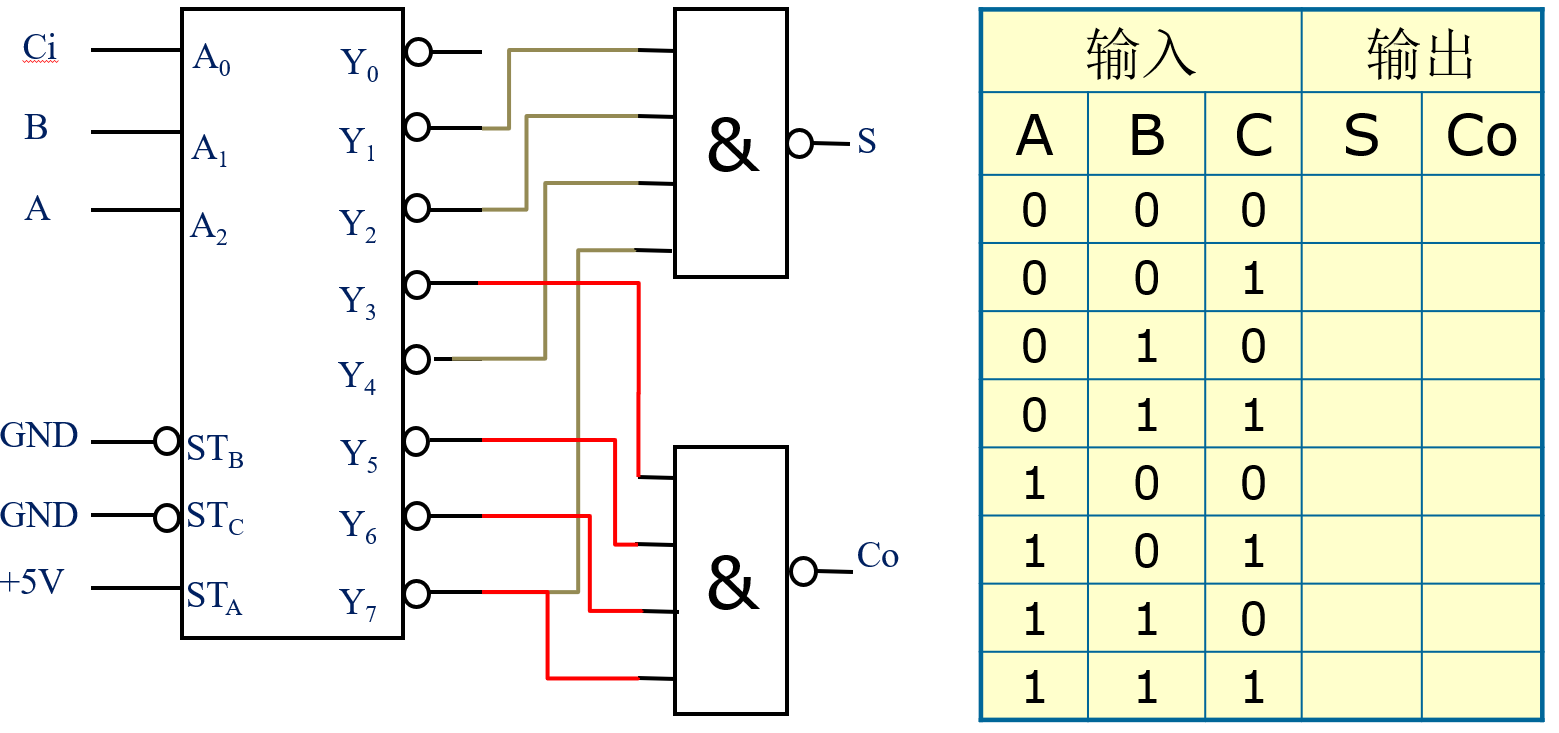
\includegraphics[scale=0.3]{8.png}
                            \label{fig:label}
                            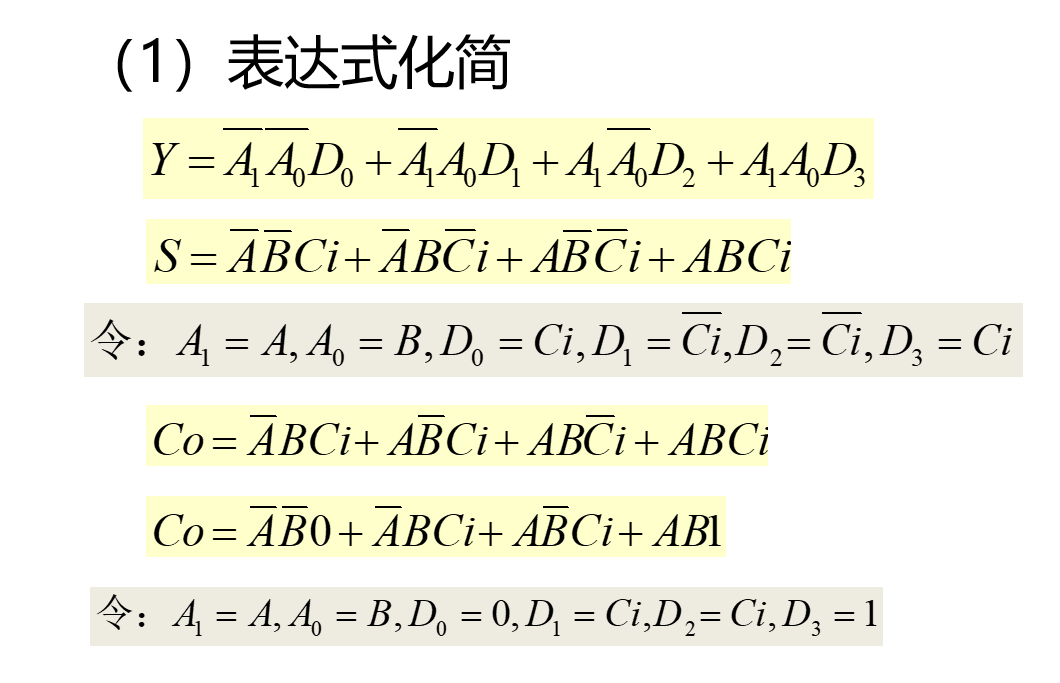
\includegraphics[scale=0.4]{11.png}
                            \label{fig:label}
                            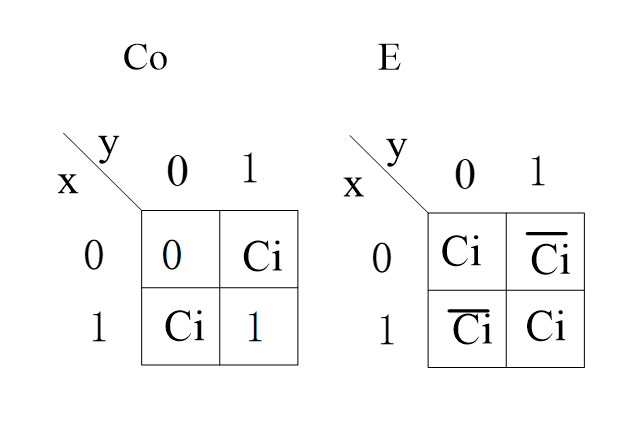
\includegraphics[scale=0.4]{12.png}
                            \label{fig:label}
                        \end{center}
                              \begin{itemize}
                                  \item [1)]  3-8译码器介绍:$74LS138$
                                  \begin{center}
                                      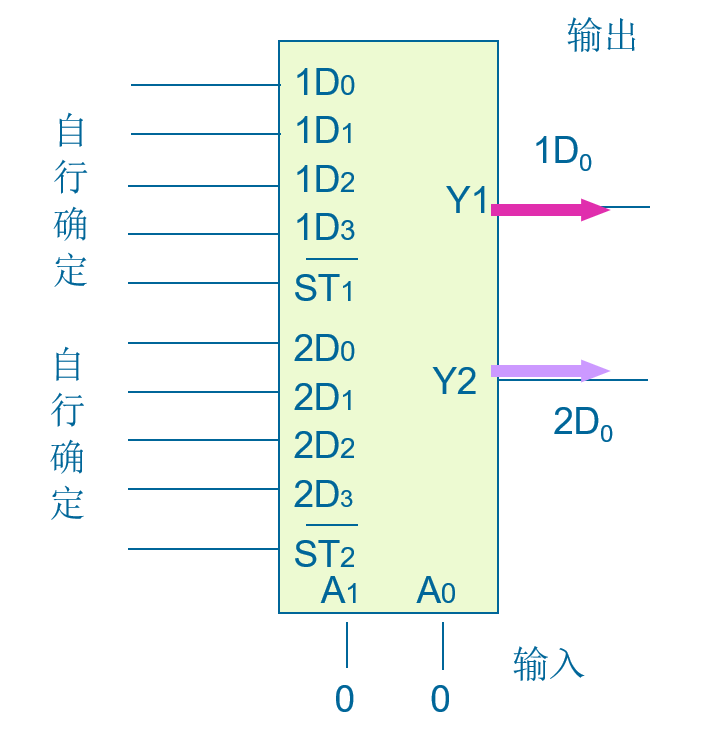
\includegraphics[scale=0.4]{10.png}
                                  \end{center}
                                  \item [2)]  双四输入与非门$74LS20$

                              \end{itemize}
                    \end{itemize}
              \item 原理及设计方案:
                    \begin{itemize}
                        \item [1.]  用MSI设计组合电路的方法:
                              \begin{center}
                                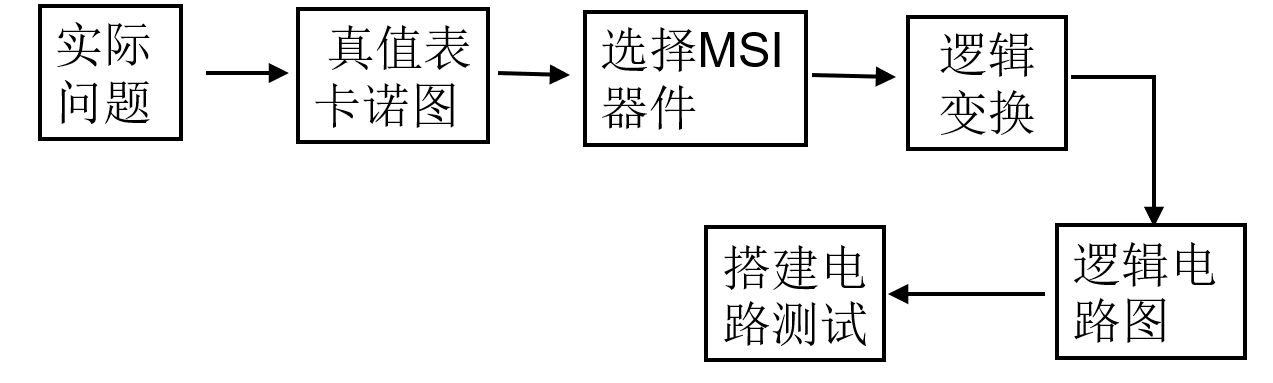
\includegraphics[scale = 0.3]{1.png}
                                \label{fig:label}
                              \end{center}
                        \item [2.]  中规模组合电路设计特点
                        
                        中规模组合电路设计和小规模组合电路设计的不同之处在于它一般不必进行太多的化简,所以设计过程简单,且电路中所用器件较少。  

                        \item [3.] 三八译码器 
                        \begin{center}
                            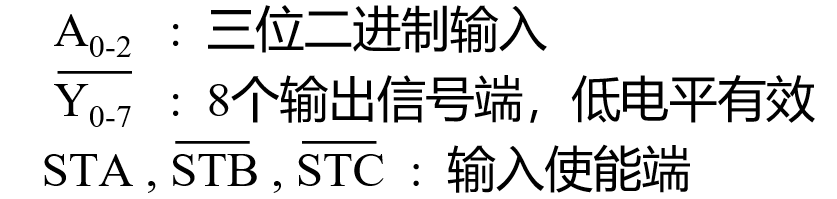
\includegraphics[scale = 0.4]{2.png}
                            \label{fig:label}
                            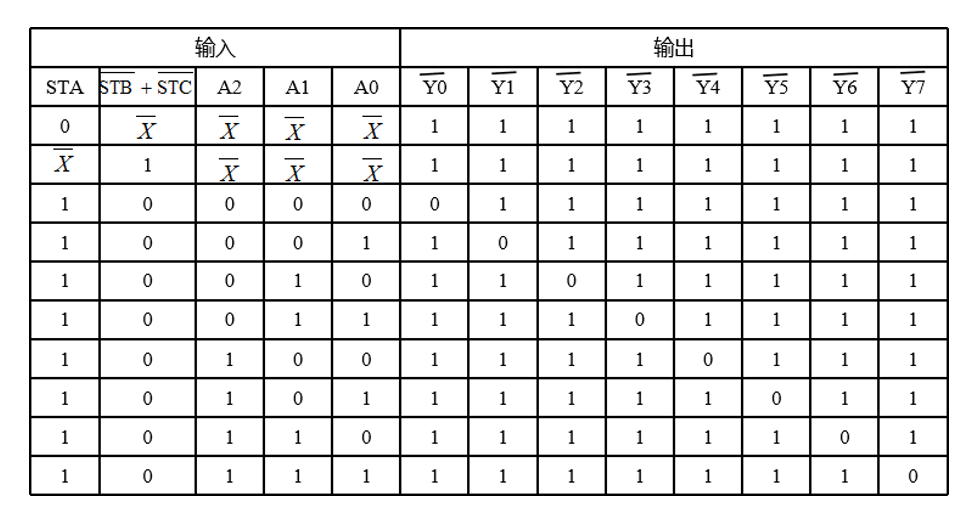
\includegraphics[scale = 0.4]{3.png}
                            \label{fig:label}
                            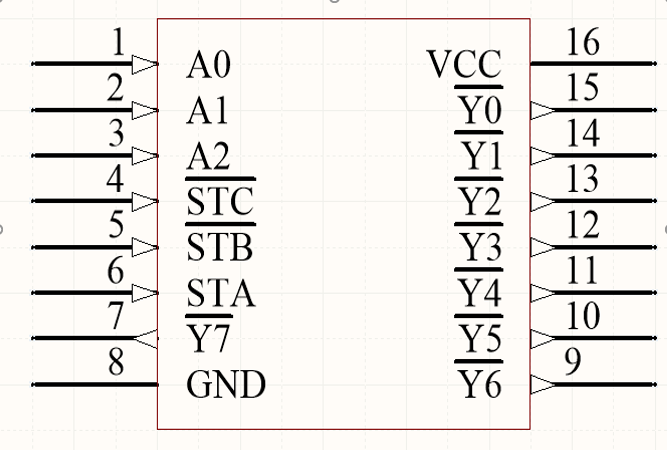
\includegraphics[scale = 0.4]{4.png}                          
                            \label{fig:label}
                        \end{center}
                        \item [4.] 数据选择器
                        \begin{center}
                            $D_{0-3}$  :  数据输入端
                            $A_{0-1}$  :  地址输入端
                            $\overline{ST}$  :  数据使能端
                            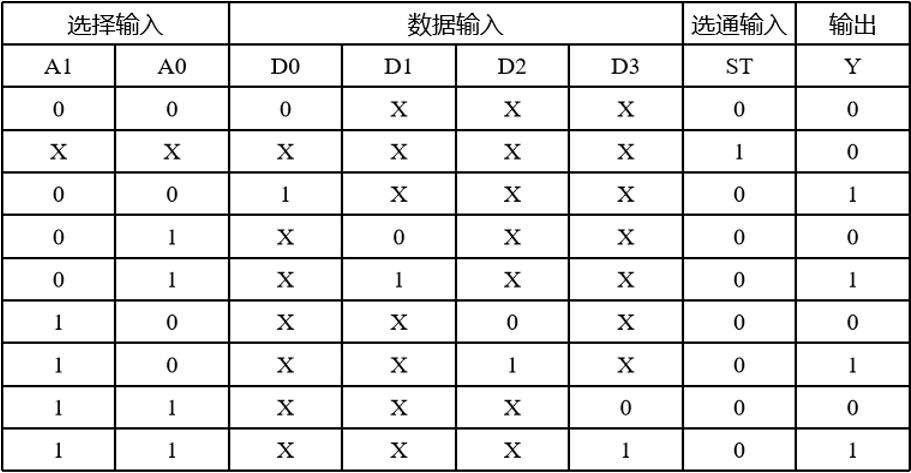
\includegraphics[scale = 0.4]{5.png}
                            \label{fig:label}
                            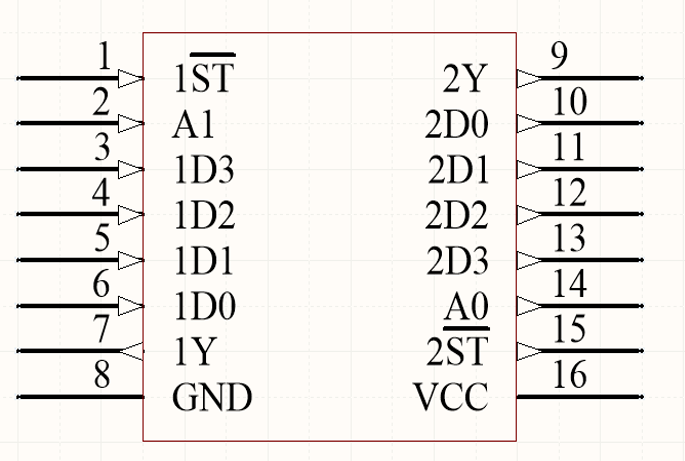
\includegraphics[scale = 0.4]{6.png}
                            \label{fig:label}
                        \end{center}
                    \end{itemize}
              \item 计算及仿真:
                    %\newpage


          \end{itemize}
    \item  实验目的:
          \begin{itemize}
              \item [1.]  掌握用MSI设计组合逻辑电路的一般方法。
              \item [2.]  加深对译码器与数据选择器的理解。
              \item [3.]  了解译码器与数据选择器的应用。 
          \end{itemize}

    \item  实验过程及数据分析:
\end{enumerate}
\end{document}